\documentclass[11pt]{article}
\usepackage[T1]{fontenc}
\usepackage{lmodern}
\usepackage{amsmath,amssymb,amsthm,mathtools}
\usepackage[margin=1in]{geometry}
\usepackage{enumitem,microtype,booktabs,graphicx}
\usepackage{xcolor,tikz}
\usetikzlibrary{arrows.meta,positioning,calc,decorations.pathreplacing}
\usepackage[hyphens]{url}
\usepackage[colorlinks=true,linkcolor=black,citecolor=blue,urlcolor=blue]{hyperref}
\usepackage[nameinlink,capitalise,noabbrev]{cleveref}
\hypersetup{pdftitle={Unconditional time lower bounds for Weisfeiler-Leman equivalence},pdfauthor={OpenAI}}

\newcommand{\F}{\mathbb{F}}
\newcommand{\N}{\mathbb{N}}
\newcommand{\Z}{\mathbb{Z}}
\newcommand{\WL}{\mathrm{WL}}
\newcommand{\AC}{\mathrm{AC}}
\newtheorem{theorem}{Theorem}[section]
\newtheorem{lemma}[theorem]{Lemma}
\newtheorem{proposition}[theorem]{Proposition}
\newtheorem{corollary}[theorem]{Corollary}
\theoremstyle{definition}
\newtheorem{definition}[theorem]{Definition}
\theoremstyle{remark}
\newtheorem{remark}[theorem]{Remark}
\numberwithin{equation}{section}
\setlist[enumerate]{itemsep=3pt,topsep=5pt}
\setlist[itemize]{itemsep=3pt,topsep=5pt}
\allowdisplaybreaks[1]

\title{Unconditional time lower bounds for\\
Weisfeiler--Leman equivalence}
\author{OpenAI}
\date{September 25, 2026}

\begin{document}
\maketitle

\begin{abstract}
For every sufficiently large fixed $k$, deciding whether two
$n$-vertex graphs are $k$-Weisfeiler--Leman equivalent requires
$n^{\Omega(k)}$ deterministic sequential time in the worst case.
The bound holds at every sufficiently large graph order, even for
simple connected uncolored graphs of diameter at most two, without a
complexity assumption. Inputs are explicit adjacency matrices; the models
are multitape Turing machines and sequential logarithmic-word RAMs with
fixed polynomial-bit-time instructions. Both joint and separate replacement
conventions are covered.
\end{abstract}

\section{Introduction}\label{sec:introduction}

The refinement method originates in Weisfeiler and Leman's work on graph
canonization \cite{WL1968}. Its higher-dimensional form assigns colors to tuples of vertices
by repeatedly recording their local extension patterns. For each fixed
dimension $k$, stabilization gives a polynomial-time test of
$k$-Weisfeiler--Leman equivalence. The direct algorithms have running
time $n^{O(k)}$: there are $n^k$ tuples, at most polynomially many
refinement rounds in their number, and each round can be implemented
in polynomial time in the tuple table. The question considered here
is whether a growing exponent is necessary for \emph{any} sequential
algorithm deciding the equivalence relation, rather than just for an
implementation of refinement.

For $k\ge2$, initial tuple colors record coordinate equalities and
adjacencies. Each refinement step retains the old color and counts
replacement colors. The \emph{joint} convention counts a multiset of
$k$-component replacement-color vectors, one vector for each new vertex
used in every coordinate; the \emph{separate} convention counts a replacement multiset
for each coordinate independently. With common color names on the two
graphs, equivalence means equality of their stable $k$-tuple color
histograms. Section~\ref{game:section} gives the full formulas and their
game characterizations.

We give an unconditional lower bound for this decision problem. Input graphs are represented
by explicit adjacency matrices. A decider is uniform
in the input size; it may depend arbitrarily on the fixed dimension
$k$. For a decider $A$, let $T_A(n)$ be its worst-case running time on
pairs of graphs having $n$ vertices each.

\begin{theorem}\label{thm:main}
There are absolute constants $c>0$ and $k_0$ with the following
property. For every fixed integer $k\ge k_0$ and every correct
deterministic decider $A$ for $k$-Weisfeiler--Leman equivalence, there
is an integer $n_0=n_0(A,k)$ such that
\[
                     T_A(n)\ge n^{ck}
             \qquad\text{for every integer }n\ge n_0.
\]
This holds for multitape Turing machines and for sequential
random-access machines with $O(\log(n+2))$-bit addresses and words,
boundedly many memory accesses per instruction, and fixed instructions
computable in time polynomial in the word length.
The same bound holds if $A$ is required to decide correctly only on
pairs of simple connected uncolored graphs of diameter at most two,
with $T_A(n)$ maximized over that class. It applies both to the
joint replacement-multiset convention for $k$-dimensional refinement
and to the separate-multiset convention defined below.
\end{theorem}

Theorem~\ref{thm:main} is unconditional; in particular, it does not
assume the Exponential Time Hypothesis. It rules out a uniform
running-time bound $f(k)n^{g(k)}$ with $g(k)=o(k)$, for any
function $f$ independent of $n$: fix a sufficiently large $k$ for
which $g(k)<ck$ and then let $n$ grow. The theorem concerns
deterministic computation, not randomized algorithms, nonuniform
advice, or unit-cost operations on unbounded integers.

The quantifiers in the theorem are important. The exponent constant $c$
is independent of both $k$ and the program. The threshold $n_0$ need not
be uniform in either. A lower bound at infinitely many graph orders would
not suffice: the conclusion excludes an algorithm that is unusually fast
at even a sparse sequence of arbitrarily large orders.

\paragraph{Historical and methodological context.}
The parity constructions of Cai, F\"urer, and Immerman established
fundamental limitations of bounded-variable graph identification
\cite{CFI1992}. Their local parity constraints and global twist obstruction
provide a basic setting for understanding why a bounded game can fail to
distinguish two globally different graphs.
Grohe, Lichter, Neuen, and Schweitzer developed compressed
Cai--F\"urer--Immerman constructions and proved, for each fixed $k\ge2$,
families requiring $\Omega_k(n^{k/2})$ rounds of $k$-dimensional
refinement \cite[Theorem~33 and Corollary~34]{CFICompression}.
Such a bound concerns the refinement process itself and does not exclude
a faster algorithm that decides its final equivalence relation by another
method. Our construction shares the use of compressed addresses and
bounded-pebble obstructions, but its individual scalar-image consistency
and exact extension properties are proved here.
Recent upper bounds on refinement iterations, including the linear bound
for classical $2$-WL of D\"oring and Neuen
\cite[Main Theorem~1]{DoeringNeuen2026}, likewise concern the refinement
procedure rather than the complexity of every equivalence decider.
A companion finite-choice reduction uses parity lifts and bounded-treewidth
homomorphism witnesses~\cite[Theorem~1.2 and Sections~2--4]{ParityLiftsWL2026}.

When the dimension is part of the input, Seppelt
\cite[Theorem~5]{Seppelt2024} and Lichter, Ra\ss mann, and Schweitzer
\cite[arXiv v2, Theorem~34]{WLDimension} proved coNP-hardness
of supplied-pair equivalence. The latter work also studies the complexity
of Weisfeiler--Leman dimension and identification.
Identification asks whether a graph is distinguished from \emph{every}
nonisomorphic graph, rather than whether a supplied pair is equivalent.
For binary-encoded input dimension $k\ge2$, joint-update supplied-pair
equivalence is EXPTIME-complete, even on connected subcubic
graphs~\cite[Theorem~1.1]{VariableDimensionWL2026}.
Input-dimension identification is separately EXPTIME-complete, using
joint updates for $k\ge2$ and ordinary color refinement at
$k=1$~\cite[Theorem~1.1]{WLIdentification2026}.
These are different quantifiers: neither identification hardness nor
hardness with the dimension as part of the input supplies the fixed-dimension time exponent of
Theorem~\ref{thm:main}.

For existential pebble games, Berkholz proved unconditional time lower
bounds with exponent linear in the number of pebbles
\cite[Theorem~1]{ExistentialPebbles}. That game asks Duplicator to
respond to an already chosen element while preserving a partial
homomorphism. The bijective-game framework goes back to
Hella~\cite{Hella1996}. In the version used here, Duplicator must first
announce a bijection, and the resulting marked correspondence must be
a partial isomorphism. We therefore prove both the game correspondence
and the complete reduction rather than treating existential-game
hardness as a black-box input. The time argument uses classical padded
diagonalization: Hennie and Stearns already used padded machine indices
and clocked full-input self-simulation in their hierarchy proof
\cite[Section~6, Theorem~7]{HennieStearns1966}. We prove the precise
every-length language and the graph-order transfer required here.

\paragraph{The proof mechanism.}
Two obstacles separate these precedents from the desired bound. First,
a polynomial-time computation with an exponent proportional to $k$
has too many addressed locations to list in a small reduction. Second,
local consistency uses symmetric comparisons, whereas a computation
must propagate information forward without forcing false predecessors
to become true. The construction addresses these obstacles separately.

Put $[m]=\{0,\ldots,m-1\}$, and fix a finite pattern of variable types
and comparisons, called the \emph{description shape}.
The main technical ingredient compresses a consistency problem with
variables indexed by $r$-tuples in $[m]^r$ into graphs with
$O_{r,\mathrm{shape}}(m^2)$ local blocks. A block records only two adjacent address
coordinates. A full ring of $r$ blocks exposes one addressed vector,
and one spare pair transports that vector's scalar image along a
constraint. Long subdivisions in the constraint direction keep every
small block collection near at most one original variable type.
The number $m$ controls the address alphabet; all vector values remain
over $\F_2$. Removing colors yields $O_{r,\mathrm{shape}}(m^6)$ vertices,
not $O(m^2)$ vertices.

The converse is the delicate part. A local translation offset specifies
how to translate every valuation in one block. We construct families of
such offsets that project \emph{exactly} onto the families for smaller
collections of blocks: every already retained assignment extends.
Auxiliary block corners carry potentials, and edges between them carry
the recorded vector or scalar values, called \emph{readouts}. A component
is \emph{nonwrapping} if every closed walk crosses a fixed seam of the
coordinate cycle an even number of times. On such a component, a change
of shift can be absorbed into corner potentials without changing the
readouts. A complete ring recovers one full address, and
individual-edge consistency supplies exactly the extension it needs.
This projection argument may be useful independently whenever
product addresses must be hidden from a bounded bijective game.

Two further ingredients connect the construction to time complexity.
A two-coordinate buffer makes scalar-image consistency simulate
directed circuit propagation without transmitting unwanted
restrictions backward. A product-indexed circuit then records a
one-tape computation using only short coordinate tables. Finally,
an explicit diagonal language is hard at \emph{every} sufficiently
large input length. Trying all padded graph sizes in a polynomial
interval transfers this fact to every sufficiently large graph
order, without assuming that an algorithm's worst-case time is
monotone in $n$.

The proof is organized around the following interfaces. In this table
$r$ and the machine are fixed while $m$ grows; $n$ is the final graph order.
\begin{center}
\small
\begin{tabular}{@{}p{0.25\textwidth}p{0.66\textwidth}@{}}
\toprule
Stage & Property retained at the next stage \\
\midrule
Bijective game & Joint $k$ uses $k+1$ pairs; separate $k$ uses $k$ pairs
  (Section~\ref{game:section}). \\
Compressed consistency & Nonempty individual scalar-image witnesses
  are equivalent to a winning $(r+1)$-pair strategy
  (Theorem~\ref{comp:reduction}). \\
Computation & Under the time and space bounds of
  Theorem~\ref{circ:computation}, acceptance is equivalent to graph
  inequivalence, with unpadded order $O(m^6)$. For sufficiently large
  $m$, padded matrices at any order $n\ge m^{20}$ cost $O(n^4)$
  to construct. \\
Diagonal language & Every one-tape decider has worst-case time greater
  than $m^s$ at every sufficiently large length
  (Theorem~\ref{diag:language}). \\
Cutoff transfer & One fast order in $[m^{20},(m+1)^{20})$ would give
  a fast decider on \emph{all} length-$m$ words
  (Section~\ref{trans:section}). \\
\bottomrule
\end{tabular}
\end{center}

All bounds in the compressed construction allow constants depending on
the fixed description shape and $r$. They do not establish a polynomial
compiler when $r$ grows with the input. Likewise, the universal hub used
to obtain diameter two has unbounded degree. No bounded-degree promise
is asserted in this paper.

\paragraph{Conventions.}
All graphs are finite. The notation $[m]$ means
$\{0,\ldots,m-1\}$, with $m\ge2$. Vector spaces, linear forms,
and potentials in the construction are over $\F_2$.
Constants may depend on a fixed parameter or machine when the
dependence is indicated by a subscript. An \emph{absolute polynomial
degree} is independent of those fixed parameters, although its
multiplicative constant and the starting size need not be.
Specific game and addressing conventions are stated before use.

\section{Weisfeiler--Leman conventions and the bijective game}
\label{game:section}

The joint refinement and its $(k+1)$-pair characterization are standard;
see Kiefer and Neuen \cite[Section~2.2 and Theorem~1]{KieferNeuen2019}.
We prove the correspondence here, including the separate convention,
to fix both the parameter shift and the order of the game moves.

Graphs in this section are finite, simple, and nonempty.  They may carry
vertex colors from a common palette; isomorphisms must preserve these
colors.  The uncolored case uses a single vertex color.  For an ordered
$k$-tuple $\bar v$ and a vertex $z$, write $\bar v[i\leftarrow z]$ for
replacement of coordinate $i$ by $z$.

\begin{definition}[The two refinement conventions]
\label{game:conventions}
Let $k\geq 2$.  The initial color $\chi_0^X(\bar v)$ records the atomic
type of $\bar v$ in $X$: all coordinate equalities, adjacencies, and vertex
colors.  The \emph{joint} convention updates by
\[
 \chi_{t+1}^X(\bar v)=
 \left(\chi_t^X(\bar v),
 \left\{\!\left\{
   \bigl(\chi_t^X(\bar v[i\leftarrow z])\bigr)_{i=1}^k
       :z\in V(X)
 \right\}\!\right\}\right).
\]
The \emph{separate} convention instead records the ordered list
\[
 \left(
 \left\{\!\left\{
   \chi_t^X(\bar v[i\leftarrow z]):z\in V(X)
 \right\}\!\right\}\right)_{i=1}^k
\]
along with the old color.  In either convention, the same recursive color
names are used for both input graphs.  Two graphs are equivalent if their
$k$-tuple color histograms agree at every round.
\end{definition}

The partitions of $V(G)^k\sqcup V(H)^k$ induced by these common color
names refine monotonically and eventually stop splitting.  Write
$\bar u\sim\bar v$ for equality of the resulting stable colors, with
the convention understood.  Thus stable histogram equality is equivalent
to equality at every round.  For the joint convention, stability gives
the following property: if $\bar u\sim\bar v$, there is a bijection
$f:V(G)\to V(H)$ such that
\begin{equation}
 \bar u[i\leftarrow z]\sim\bar v[i\leftarrow f(z)]
 \quad\text{for every }z\in V(G)\text{ and every }i\in\{1,\ldots,k\}.
 \label{game:joint-extension}
\end{equation}
Indeed, match equal members of the two finite multisets of replacement
color vectors.  For the separate convention, the same conclusion holds
for a specified coordinate $i$, with a bijection $f_i$ allowed to depend
on $i$.  An induction on the round also shows that $\sim$ is preserved
by simultaneous permutations of the coordinates.

\begin{definition}[Bijective game]
\label{game:definition}
The bijective game with $K$ pairs is played on $G,H$ as follows.  Spoiler
may remove any marked pairs and choose a vacant pair.  Duplicator then
announces a bijection $f:V(G)\to V(H)$, after which Spoiler chooses
$z\in V(G)$ and marks $z,f(z)$ with that pair.  Duplicator loses as soon
as the marked correspondence fails to preserve equality, adjacency, or
vertex colors.  A winning strategy for Duplicator must survive every
finite continuation, and hence every infinite play.  If the graph orders
differ, Duplicator cannot announce a bijection and loses.
\end{definition}

A winning position remains winning after pairs are removed: Duplicator
may retain the removed pairs privately and use the original strategy,
forgetting a private pair if its label is reused. The public position
is always a restriction of the simulated winning position.

\begin{lemma}[Exact stable equivalence]
\label{game:wl}
For the joint convention put $K=k+1$, and for the separate convention put
$K=k$.  For graphs of equal positive order the following hold.
\begin{enumerate}
 \item Two $k$-tuples have the same stable color if and only if
 Duplicator has a winning $K$-pair strategy from the position marking
 those tuples on $k$ corresponding pairs.
 \item The graphs have equal stable $k$-tuple color histograms if and
 only if Duplicator has a winning $K$-pair strategy from the empty
 position.
\end{enumerate}
\end{lemma}

\begin{proof}
First use the joint convention.  Maintain full $K$-tuples whose every
$k$-coordinate projection has equal stable colors; entries in vacant
slots are virtual.  A pair of related $k$-tuples can be extended to such
full tuples by choosing any $z$ and using
\eqref{game:joint-extension}: the projection omitting the new slot is
the original tuple, and every other projection is a replacement, up to
a simultaneous coordinate permutation.

To fill a vacant slot, apply \eqref{game:joint-extension} to the other
$k$ slots.  The announced bijection preserves the invariant for every
choice by Spoiler.  Removing pebbles simply makes their entries virtual.
Because $k\geq2$, every pair of marked entries belongs to some
$k$-coordinate projection, so the invariant implies partial
isomorphism.  This proves the forward implication in the tuple
statement.  Equal histograms supply a related pair of $k$-tuples, from
which the same construction starts with all entries virtual.

Conversely, from any winning position with $k$ marked pairs, prove by
induction on $t$ that the two tuples have equal colors at round $t$.
The case $t=0$ is partial isomorphism.  For the inductive step, ask to
use the spare pair.  For every selection $z$, retain the new pair and
discard any one of the original pairs.  The resulting $k$-pair position
is still winning, and its round-$t$ colors agree by induction.
The same announced bijection works for all discarded coordinates;
therefore the joint replacement multisets agree.

For the separate convention maintain a related full $k$-tuple, again
using virtual entries in vacant slots.  Fill slot $i$ with the bijection
$f_i$ supplied by its separate replacement multiset.  The resulting full
tuple remains related, and hence gives partial isomorphism.  For the
converse induction, remove pair $i$ and replace it using the winning
strategy.  This gives exactly the equality of replacement multisets
needed in coordinate $i$.

Finally, from an empty-position winning strategy, place the $k$ pairs
in a fixed order.  The successive announced bijections induce a
bijection $V(G)^k\to V(H)^k$: for a proposed image tuple, invert the
bijection at the first slot, then the bijection determined by that
prefix at the second slot, and continue.  Every matched pair of tuples
has equal colors at every round by the preceding induction.  Their
histograms therefore agree in either convention.
\end{proof}

The joint convention and its $(k+1)$-pair characterization are standard;
see, for example, \cite[Lemma~2]{CFICompression} and
\cite[arXiv v2, Lemma~7]{WLDimension}.  The proof above fixes explicitly the
infinite-game convention needed here.  A strategy can also be used in
reverse: announce the inverse bijection and translate Spoiler's selected
vertex through it.  Thus restricting Spoiler to select vertices in the
first graph does not change the winning relation.

\begin{lemma}[Pure tuples in a disjoint union]
\label{game:union}
Suppose $k\geq3$ and $G,H$ are connected graphs of diameter at most two.
Run either convention on $D=G\sqcup H$, including mixed tuples.  The
stable color histograms restricted to the pure tuples $V(G)^k$ and
$V(H)^k$ are equal if and only if the separate-input histograms from
Definition~\ref{game:conventions} are equal.
\end{lemma}

\begin{proof}
Stable colors in $D$ determine, for each two coordinates $u,v$, whether
\[
 u=v\quad\text{or}\quad E(u,v)\quad\text{or}\quad
 \exists z\,\bigl(E(u,z)\wedge E(z,v)\bigr).
\]
For the existential clause, replace a third coordinate and inspect its
two adjacencies in the atomic information retained by the replacement
colors.  This works for both update conventions.  By the diameter
assumption, the displayed condition is exactly membership in the same
component of $D$.

Take two related pure tuples, one in each component.  A replacement
leaves another coordinate as an anchor.  Consequently a stable-color
witness bijection on $D$, whether joint or for a specified slot, maps
replacement vertices in $G$ into $H$ and replacement vertices in $H$
into $G$.  Its restriction is a bijection $V(G)\to V(H)$.  Equal pure
histograms supply initial related tuples, and these restricted
bijections give exactly the invariant proof of
Lemma~\ref{game:wl}.  Hence Duplicator wins between $G$ and $H$.

Conversely, let Duplicator win between $G$ and $H$.  Play on $D$ against
itself by swapping the two components: use that strategy on vertices
selected in $G$ and its reverse on vertices selected in $H$.  After
any discards, each component has at most $K-1$ pairs when a new pair is
requested.  Both local strategies may therefore propose a bijection;
announce their union and commit the move only in the selected
component.  Cross-component entries have neither equality nor
adjacency on either side, so this is a winning strategy on $D$.
The successive-bijection argument in Lemma~\ref{game:wl} now matches
$V(G)^k$ bijectively with $V(H)^k$ while preserving stable colors in
$D$.  This proves equality of the pure histograms.
\end{proof}

\begin{remark}[Parameter used by the construction]
\label{game:parameter}
The remainder of the proof uses $K=r+1$ pairs and assumes $r\geq3$.
Under the joint convention $r=k$; under the separate convention
$r=k-1$.  Thus a query occupying $r$ pairs has exactly one spare pair
for transferring it.  The final graphs have a universal hub, so
Lemma~\ref{game:union} also applies to the convention that compares
pure tuples inside their disjoint union.
\end{remark}

\section{A compressed graph representation of arc consistency}
\label{comp:section}

Throughout this section, $r\geq 3$, $K=r+1$, and all vector spaces and
affine maps are over $\F_2$.  The construction stores only two consecutive
coordinates of an address in each block.  A complete address becomes
visible to the game through a ring of $r$ blocks.  A close structural
parallel appears in the compressed CFI construction of Grohe, Lichter,
Neuen, and Schweitzer: row periods involving neighboring moduli compress
a product-length cylindrical grid.  In the periodic lift, their separator
lemmas show, under their stated hypotheses, that changing one row
representative changes the unique separator meeting every row once in at
most one vertex
\cite[Section~5, Lemmas~19, 29, and~30]{CFICompression}.  The scalar-image
consistency and exact offset-extension properties used here are proved below.

\subsection{The consistency instance}

Put $[m]=\{0,\ldots,m-1\}$, where $m\geq 2$.  Fix a finite collection
$\mathcal P$ of \emph{real types}, with a dimension $d_P$ for each
$P\in\mathcal P$.  The variables
of type $P$ are indexed by $\mathbf a\in[m]^r$ and take values in
$\F_2^{d_P}$.  An \emph{edge schema} $e$ specifies ordered endpoint types
$P,R$, possibly equal, together with the following data:
\begin{itemize}
\item For each coordinate $i$, a set $A_{e,i}\subseteq[m]$ and an injection
  $\sigma_{e,i}\colon A_{e,i}\longrightarrow[m]$.
\item An affine form $\phi_{e,0}(u)=\lambda_{e,0}u+d_{e,0}$ at $P$ and
  an affine form $\phi_{e,1}(u)=\lambda_{e,1}u+d_{e,1}$ at $R$.
\end{itemize}
The forms are scalar valued; their linear parts may be zero.  Write
$A_e=\prod_i A_{e,i}$ and
$\boldsymbol\sigma_e(\mathbf a)=(\sigma_{e,i}(a_i))_{i=1}^r$.
For every $\mathbf a\in A_e$, the schema gives one individual comparison
between $\phi_{e,0}$ at $(P,\mathbf a)$ and $\phi_{e,1}$ at
$(R,\boldsymbol\sigma_e(\mathbf a))$.

\begin{definition}\label{comp:ac}
The instance has \emph{individual-edge arc consistency} if there are
nonempty sets $Q_{P,\mathbf a}\subseteq\F_2^{d_P}$, for every real type
and every address, such that
\begin{equation}\label{comp:ac-equation}
 \phi_{e,0}(Q_{P,\mathbf a})
 =\phi_{e,1}(Q_{R,\boldsymbol\sigma_e(\mathbf a)})
 \qquad(e,\ \mathbf a\in A_e).
\end{equation}
Each equality is imposed separately.  In particular, parallel comparisons
are not combined into a single relation.
\end{definition}

This is a per-comparison local-support condition, in the tradition of arc
consistency \cite[Section~4]{Mackworth1977}. Every possible value at one
endpoint must have a supporting value at the other, but the support may
depend on the value and on the comparison. Even when a schema has the
same type and address at both ends, its two endpoint occurrences may
use different vectors from the same set. We do not ask for one globally
compatible vector at every address.

A \emph{description shape} fixes the types, their dimensions, and the
number and incidence of the schemas.  The coordinate sets and maps can
depend on $m$.  They are specified by their one-coordinate tables.
The scalar forms may vary as well, but their descriptions have bounded
size because the dimensions and number of schemas are fixed.

\begin{theorem}[Compressed consistency reduction]\label{comp:reduction}
For fixed $r$ and fixed description shape, an instance as above determines
two equally large simple uncolored connected graphs $G^0,G^1$, of
diameter at most two and order
\[
                         O_{r,\mathrm{shape}}(m^6),
\]
such that Duplicator wins the $K$-pair bijective game on $G^0,G^1$ if and
only if the instance has individual-edge arc consistency.
The construction uses the bounded scalar-form data together with the
one-coordinate tables, and enumerates $O_{r,\mathrm{shape}}(m^2)$ blocks
without enumerating all full addresses.
An arbitrary equal number of additional vertices can be added to the two
graphs while preserving the equivalence, connectedness, and diameter
bound.
\end{theorem}

We prove the theorem in several steps.  An unused real type of dimension
one may be added at the outset.  This does not affect consistency and
ensures that the constructions below have at least two valuation vertices.

\subsection{Subdivided types and local blocks}

Replace each schema by a path with $4(r+1)$ private internal types, each
of dimension one.  Call this subdivided path a \emph{wire}; its endpoints
are the original real types, and its segments are \emph{links}.
At an internal type of schema $e$,
the allowed labels in coordinate $i$ are $A_{e,i}$; at a real type all
labels in $[m]$ are allowed.  Along the path the coordinate matches are
identity matches on these allowed labels, except at the second real
endpoint, where the match is $p\mapsto\sigma_{e,i}(p)$.

For a link $\ell$ with endpoints $t,u$, its scalar comparison has the form
\begin{equation}\label{comp:link}
                         L_{\ell,t}h_t+L_{\ell,u}h_u=b_\ell.
\end{equation}
The notation for a linear form is local to its link and endpoint.  An
internal link has both forms equal to the identity and $b_\ell=0$.
At a real endpoint use the linear part of its original affine form,
identity at the internal endpoint, and the constant term as $b_\ell$.
Thus the internal scalar carries the value of the original affine form.
For use only in the analysis, extend each coordinate injection to a
permutation of $[m]$; the actual links retain only their allowed matches.

Boundary indices $i=1,\ldots,r$ are cyclic, with $r+1$ denoting boundary
$1$.  Put $\delta_i=1$ for $i=r$ and $\delta_i=0$ otherwise.  A
\emph{corner} is a triple $(i,t,p)$, where $p$ is an allowed label at
boundary $i$ of type $t$.  We use two kinds of blocks.
\begin{itemize}
\item A \emph{site block} at type $t$, row $i$, and allowed labels $p,p'$
  has one vector readout $x\in\F_2^{d_t}$.  Its name is the horizontal
  edge from $(i,t,p)$ to $(i+1,t,p')$.  All values are allowed.
\item A \emph{square block} at link $\ell=tu$, row $i$, and allowed
  matches at boundaries $i,i+1$ has the two corresponding horizontal
  readouts $x_t,x_u$ and two scalar vertical readouts $y_i,y_{i+1}$.
  A vertical readout is named by its boundary, link, and label match.
  In version $\varepsilon\in\{0,1\}$ the permitted valuations satisfy
  \begin{equation}\label{comp:square}
   L_{\ell,t}x_t+L_{\ell,u}x_u+y_i+y_{i+1}
                           =\varepsilon\delta_i b_\ell.
  \end{equation}
\end{itemize}
Version $0$ is called homogeneous and version $1$ affine.  Two occurrences
of a readout with the same name denote the same vector or scalar.  A
\emph{valuation} of a block specifies all its readouts.  The legal
valuations of any block form a linear space in version $0$ and a
nonempty affine coset of that space in version $1$.  For a square this
follows, for example, from the coefficient one of $y_i$ in
\eqref{comp:square}.

For the moment, construct vertex-colored graphs: the vertices are legal
block valuations, and each block has its own color.  Between two distinct
blocks sharing at least one readout name, place an edge exactly when
the valuations agree on \emph{all} their shared readouts.  There are no
other edges.  Corresponding blocks have equally many vertices in the
two graphs.

\begin{figure}[htbp]
\centering
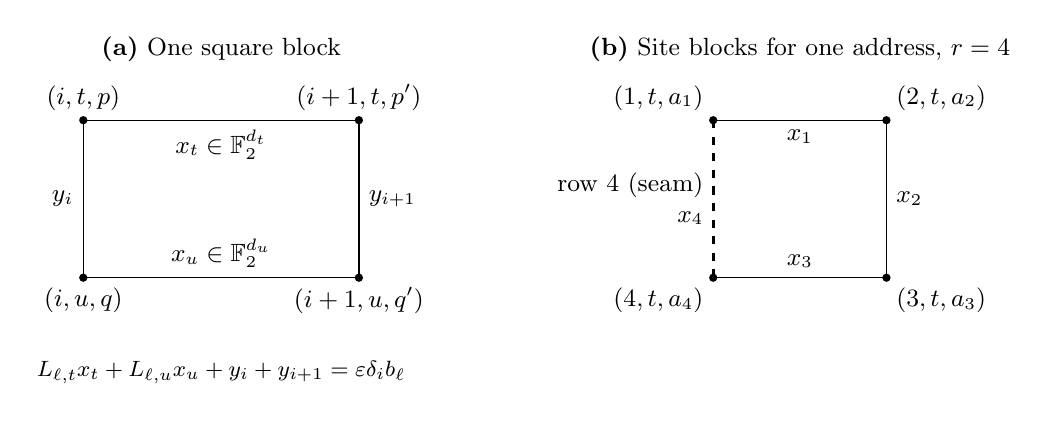
\begin{tikzpicture}[font=\small,line width=0.5pt]
  \node at (1.75,0.9) {\textbf{(a)} One square block};
  \draw (0,0) -- (3.5,0) -- (3.5,-2) -- (0,-2) -- cycle;
  \fill (0,0) circle (1.5pt);
  \fill (3.5,0) circle (1.5pt);
  \fill (3.5,-2) circle (1.5pt);
  \fill (0,-2) circle (1.5pt);
  \node[above] at (0,0) {$(i,t,p)$};
  \node[above] at (3.5,0) {$(i+1,t,p')$};
  \node[below] at (0,-2) {$(i,u,q)$};
  \node[below] at (3.5,-2) {$(i+1,u,q')$};
  \node[below] at (1.75,0) {$x_t\in\F_2^{d_t}$};
  \node[above] at (1.75,-2) {$x_u\in\F_2^{d_u}$};
  \node[left] at (0,-1) {$y_i$};
  \node[right] at (3.5,-1) {$y_{i+1}$};
  \node[font=\footnotesize] at (1.75,-3.2)
    {$L_{\ell,t}x_t+L_{\ell,u}x_u+y_i+y_{i+1}
       =\varepsilon\delta_i b_\ell$};

  \node at (9.1,0.9) {\textbf{(b)} Site blocks for one address, $r=4$};
  \draw (8,0) -- (10.2,0) -- (10.2,-2) -- (8,-2);
  \draw[dashed,very thick] (8,-2) -- (8,0);
  \fill (8,0) circle (1.5pt);
  \fill (10.2,0) circle (1.5pt);
  \fill (10.2,-2) circle (1.5pt);
  \fill (8,-2) circle (1.5pt);
  \node[above left] at (8,0) {$(1,t,a_1)$};
  \node[above right] at (10.2,0) {$(2,t,a_2)$};
  \node[below right] at (10.2,-2) {$(3,t,a_3)$};
  \node[below left] at (8,-2) {$(4,t,a_4)$};
  \node[below] at (9.1,0) {$x_1$};
  \node[right] at (10.2,-1) {$x_2$};
  \node[above] at (9.1,-2) {$x_3$};
  \node[left,align=right] at (8,-1) {row $4$ (seam)\\$x_4$};
\end{tikzpicture}
\caption{Corner and readout geometry.  Dots are corners; each vertex
of a valuation graph is a legal valuation of an entire block.
In (a), horizontal edges name vector readouts and vertical edges name
scalar readouts for the two allowed label matches.  Each horizontal
edge also specifies its corresponding site block.
In (b), a fixed type and allowed address $(a_1,a_2,a_3,a_4)$ select
four separate site blocks, with row $4$ crossing the cyclic seam.
All four edges in (b) name site readouts.  Blocks share a readout
through a common named edge; meeting only at a corner does not suffice.}
\label{comp:readout-figure}
\end{figure}

\subsection{Reading a comparison}

\begin{lemma}\label{comp:necessity}
A block-preserving winning strategy with $r+1$ pairs implies
individual-edge arc consistency.
\end{lemma}
\begin{proof}
Spoiler always selects zero valuations in the homogeneous graph.  They
are legal in every block.  Whenever two pebbled distinct blocks share
readouts, their selected zero valuations are adjacent, so their answers
must agree on every shared readout.

We may regard a finite query as ending immediately after discards, by
the removal closure of winning positions from Section~\ref{game:section}.

Fix a type $t$ and an allowed full address.  Its \emph{site ring} consists
of the $r$ site blocks using the address labels at consecutive boundaries,
as illustrated in Figure~\ref{comp:readout-figure}(b).
The sum of their answered horizontal readouts is a value
$h_t\in\F_2^{d_t}$.  To cross a link at a matched address, replace these
site blocks by their corresponding square blocks, one row at a time:
place the square while retaining its old site, and then discard the
site.  This uses at most $r+1$ pairs and preserves each old horizontal
readout on the $t$ side.  When all $r$ squares are pebbled, their vertical
readouts agree at adjacent boundaries.  Summing \eqref{comp:square} in
the affine graph gives \eqref{comp:link} for the sums on the two sides.
Now replace the squares, in the same manner, by the site ring at $u$.
Its sum is preserved from the $u$ side of the squares.  Repeating along
the subdivided path transmits the original affine comparison.  The same
procedure works in reverse.

Fix a winning strategy.  Let $Q_{P,\mathbf a}$ consist of all sums
attainable on the real site ring $(P,\mathbf a)$ in plays consistent with
that strategy, with zeros selected on the homogeneous side and all other
pairs discarded.  These sets are nonempty: Spoiler can always query any
such ring from the empty position.  Starting with any attainable endpoint
sum and transmitting across an individual edge produces an attainable
sum at its other endpoint with the same affine image.  Transmitting in
both directions proves both inclusions in \eqref{comp:ac-equation}.
\end{proof}

\subsection{Corner graphs and wrapping}

For a set $U$ of blocks, let $\Gamma_U$ be the graph on all their corners,
with their named horizontal and vertical edges.  Each block is connected
in this graph and therefore belongs to a single component.  The
\emph{type support} of a component consists of the types and links used
by its blocks, viewed in the subdivided type multigraph.

\begin{lemma}\label{comp:support}
If $|U|\leq r+1$, every component's type support is a tree containing at
most one real type.  With no real type it lies in the interior of one
wire; with a real type it consists of that type and short arms of
incident wires.
\end{lemma}
\begin{proof}
The support is connected and uses at most $r+1$ distinct links, since
each square contributes one link.  Every subdivided wire has
$4(r+1)+1$ links.  Reaching two real types, or closing a cycle in the
support, would require traversing an entire wire.  This also applies to
a subdivided original loop or to a cycle arising from parallel schemas.
Internal types are private to their wires, giving the remaining claims.
\end{proof}

Choose a reference type in such a support.  At each boundary, use the
extended coordinate permutations along its tree paths to align all
labels with labels at the reference type.  Actual vertical edges then
preserve the aligned label.  On a connected subtree, these alignments
restrict consistently, up to the choice of reference type.

A collection of blocks is \emph{wrapping} if its corner graph has a
closed walk traversing an odd number of horizontal edges in row $r$,
counted with multiplicity.
The site ring in Figure~\ref{comp:readout-figure}(b) is one example
of a wrapping witness, not a classification of all witnesses.

\begin{lemma}[Address recovery]\label{comp:wrapping}
For block sets contained in a set $U$ of size at most $r+1$:
\begin{enumerate}
\item Every wrapping collection has at least $r$ blocks.
\item A wrapping collection of size $r$ has one block in every row,
  all in one component, and determines a consistent full address in
  the aligned coordinates of that component's type support.
\item All wrapping subcollections of $U$ of size $r$ lie in one
  component and determine the same aligned full address.
\end{enumerate}
\end{lemma}
\begin{proof}
For any closed walk, the parity of its horizontal traversals is the same
in each row.  Indeed, at each boundary the total incidence parity is
zero, while vertical traversals contribute twice at that boundary.
Odd seam parity therefore requires an odd number of traversals in every
row and hence at least one block in every row.

With exactly $r$ blocks, there is one per row, and the witnessing walk
meets them all.  All horizontal edges of the block in a given row have
the same pair of aligned labels.  At boundary $i$, apply parity
conservation separately at each aligned label, combining all types.
Vertical edges preserve that label.  Since both incident rows have odd
traversal parity, their specified labels at boundary $i$ must agree.
These labels give the full address.

Two size-$r$ subcollections of $U$ share at least $r-1$ blocks in distinct
rows.  They therefore overlap, and lie in one component.  They can differ
only in the remaining row.  Every boundary has an incident common row
when $r\geq3$, so the recovered addresses agree in every coordinate.
\end{proof}

We impose full-address restrictions only when a size-$r$ subcollection
wraps.  This is the information that can persist in the at most $r$
occupied blocks before a new game move.  A collection first wrapping at
$r+1$ blocks receives no such restriction: its proper subsets are
nonwrapping, and the potential adjustment below will let their shifts
change without altering their readouts.

\subsection{Compatible families of offsets}

Assume now that \eqref{comp:ac-equation} holds.  For an internal type of
wire $e$ and an allowed address $\mathbf a\in A_e$, define its scalar set
to be
\begin{equation}\label{comp:internal-q}
 Q_{t,\mathbf a}
   =\phi_{e,0}(Q_{P,\mathbf a})
   =\phi_{e,1}(Q_{R,\boldsymbol\sigma_e(\mathbf a)}).
\end{equation}
This is nonempty and the same at all internal types of that wire, whose
labels use its first address system.

For every block set $U$ with $|U|\leq r+1$, we construct a nonempty family
$\mathcal H_U$ of compatible affine valuations of those blocks.  These
valuations will serve as \emph{offsets} for translations; they need not
be the actual vertices currently selected by Spoiler or Duplicator.
The construction below represents an offset assignment by component
shifts and corner potentials.  A member of $\mathcal H_U$ retains only
the resulting readout values, and may have more than one representation.

For each component $C$ of $\Gamma_U$, independently choose a vector
$h_t\in\F_2^{d_t}$ for every type in its support, satisfying
\eqref{comp:link} on every support link.  If $C$ contains a wrapping
subcollection of size $r$, impose one additional condition at its address
from Lemma~\ref{comp:wrapping}:
\begin{itemize}
\item If the support contains a real type $P$, require
  $h_P\in Q_{P,\mathbf a}$, expressing the address at $P$.
\item Otherwise, require its common internal scalar to belong to
  $Q_{t,\mathbf a}$, expressing the address in that wire's system.
\end{itemize}
In the second case the address is allowed for the entire wire: every
coordinate is read by a block of the wrapping collection at an internal
type, where it belongs to $A_{e,i}$.  In the first case real addresses
are unrestricted.  In particular, an incomplete arm out of $P$ need
not allow that full address.

Call a shift family satisfying the link equations and the applicable
$Q$ condition \emph{admissible}.  On an interior support it is
parameterized by one common scalar.  On a support with a real type,
it is parameterized by its one real vector: the scalar on each arm is
the corresponding endpoint affine form of that vector, constant down
the arm.  Admissible shifts therefore exist, since the required $Q$
sets are nonempty; when no $Q$ condition is imposed, the parameter is
arbitrary.  For an original loop, its two short arms are treated
separately; the support cannot traverse the interior connecting them.

Choose an arbitrary potential $M_v\in\F_2^{d_t}$ at each corner $v$ of
type $t$.  Define the readouts by
\begin{align}
 x_{vw}&=M_v+M_w+\delta_i h_t
   &&\text{on a horizontal edge in row $i$ at type $t$},
   \label{comp:potential-x}\\
 y_{vw}&=L_{\ell,t}M_v+L_{\ell,u}M_w
   &&\text{on a vertical edge of link $\ell=tu$}.
   \label{comp:potential-y}
\end{align}
Let $\mathcal H_U$ be all assignments obtained this way.  Substitution
in a square cancels every potential term, leaving
$\delta_i(L_{\ell,t}h_t+L_{\ell,u}h_u)=\delta_i b_\ell$.
Thus every assigned valuation is legal in the affine graph, and readouts
with the same name agree.  The family is nonempty, including for
$U=\varnothing$.

For a site ring at type $t$ and address $\mathbf a$, write
$M_i=M_{(i,t,a_i)}$ and $M_{r+1}=M_1$.  Its compatible offset
readouts from \eqref{comp:potential-x} satisfy
\[
 \sum_{i=1}^r x_i
 =\sum_{i=1}^r\bigl(M_i+M_{i+1}+\delta_i h_t\bigr)
 =h_t.
\]
Each corner potential occurs twice, and row $r$ contributes the
component shift $h_t$.

Nonemptiness alone is not enough for the game.  When $V$ is the set of
retained blocks, every readout in its chosen offset assignment
$a_V\in\mathcal H_V$ must be kept when a new block is added.  Its
representing shifts and potentials may change.  A retained wrapping
component constrains its shift; on the other components we will absorb
shift changes into the potentials.  The next lemma gives exact extension,
so a separate extension can be chosen for each prospective new block.

\begin{lemma}[Exact projection]\label{comp:projection}
For $V\subseteq U$ with $|U|\leq r+1$,
\begin{equation}\label{comp:projection-equation}
                         \mathcal H_U\big|_V=\mathcal H_V.
\end{equation}
\end{lemma}
\begin{proof}
If $V=U$ there is nothing to prove.  Assume $V\subsetneq U$, so
$|V|\leq r$.  If a component of $\Gamma_V$ wraps,
Lemma~\ref{comp:wrapping} requires at least $r$ blocks.  It therefore
uses all $r$ blocks of $V$, and there is at most one such component.

\emph{Admissible shifts on a retained wrapping component.}
Let $D$ be a wrapping component of $\Gamma_V$, contained in a component
$C$ of $\Gamma_U$.  Compare all recovered addresses in the alignment
of $C$'s support.  The size-$r$ witness in $D$ is also in $C$, so
Lemma~\ref{comp:wrapping} gives the same address for $D$ and for the
$Q$ condition on $C$.  We claim that restricting admissible shift
families from $C$ to $D$ gives exactly all admissible shift families
on $D$.
\begin{itemize}
\item If both supports contain a real type, it is the same type with
  the same $Q$ restriction.  Its real vector determines every arm
  scalar in either support.  Every allowed old vector therefore
  extends by assigning the newly present arm scalars.
\item If $C$ contains no real type, both supports lie in the same
  wire interior.  They are parameterized by the same common scalar
  with the same $Q$ restriction, so restriction is exact.
\item If only $C$ contains a real type, $D$ lies inside one arm of a
  wire $e$ with ordered real endpoints $P,R$.  Write its internal
  address as $\mathbf a\in A_e$.  The internal coordinates use the
  first endpoint's system.  Since every $a_i\in A_{e,i}$, the permutation
  extending $\sigma_{e,i}$ sends $a_i$ to the actual matched label
  $\sigma_{e,i}(a_i)$, and its inverse returns that label to $a_i$.
  All other matches along the wire are identities.
  Thus the recovered address is $\mathbf a$ at the first endpoint $P$
  and $\boldsymbol\sigma_e(\mathbf a)$ at the second endpoint $R$.
  Equation~\eqref{comp:internal-q} gives
  \[
   \phi_{e,0}(Q_{P,\mathbf a})
   =Q_{t,\mathbf a}
   =\phi_{e,1}(Q_{R,\boldsymbol\sigma_e(\mathbf a)}).
  \]
  Using the equality for the endpoint reached by $C$, every admissible
  old scalar has an admissible real preimage, and every admissible real
  vector restricts to an admissible old scalar.  After choosing the real
  preimage, assign the scalars on the other arms from that vector.
  These remain separate endpoint statements when $P=R$.
\end{itemize}
These cases are exhaustive, since a real type in $D$ also belongs to $C$.

\emph{Restriction of readouts.}
Take a member of $\mathcal H_U$ and one representation by shifts and
potentials.  Restrict both to each component $D$ of $\Gamma_V$.
The link equations remain valid.  If $D$ wraps, the shift fact just
proved preserves its $Q$ condition; if $D$ does not wrap, it has no
such condition.  Formulas~\eqref{comp:potential-x} and
\eqref{comp:potential-y} then give the same readouts on $V$.
Hence $\mathcal H_U|_V\subseteq\mathcal H_V$.

\emph{Extension of retained readouts.}
Fix $a_V\in\mathcal H_V$ and choose one representation, writing
$h_t^D$ for its shifts on an old component $D$ and $M_v$ for its corner
potentials.  On each new component $C$ choose admissible shifts
$\widehat h_t^C$.  If $C$ contains the wrapping old component, choose
these shifts to agree with $h_t^D$ throughout that old support; the
shift fact makes this possible.  Since a wrapping old component uses
all $r$ blocks of $V$, no new real shift must lift two independently
prescribed old arm scalars.

The new shifts already agree on a wrapping $D$.  On each nonwrapping
$D$ we now adjust the representing potentials so that the new shifts
produce the original readouts of $a_V$.  Mark each horizontal edge in
row $i$ with $\delta_i$ and each vertical edge with zero.  Every closed
walk in $D$ has mark sum zero.  Summing marks along paths from a root
therefore defines bits $s_v$ such that $s_v+s_w$ is the mark of every
edge $vw$.

For a type $t$ of this $D\subseteq C$, put
$g_t=h_t^D+\widehat h_t^C$, the difference of its old and new shifts
over $\F_2$.  Both shift families satisfy the same affine link
equations, so
\[
                         L_{\ell,t}g_t=L_{\ell,u}g_u
\]
on every support link.  Replace the old corner potentials of type $t$
by $M'_v=M_v+s_vg_t$.  Including the change of shift, the change in a
horizontal readout from \eqref{comp:potential-x} is
\[
                  (s_v+s_w)g_t+\delta_i g_t=0.
\]
For a vertical edge, $s_v=s_w$, so the change in its readout from
\eqref{comp:potential-y} is
\[
                  s_vL_{\ell,t}g_t+s_wL_{\ell,u}g_u=0.
\]
Thus every old readout is preserved.

Perform this adjustment independently on each nonwrapping component,
and keep the old potentials on a wrapping component.  Distinct old
components have disjoint corner sets, even if their type supports share
types or the new blocks merge them.  Their potential assignments
therefore do not conflict.  Assign arbitrary potentials to new corners
of $\Gamma_U$.  Together with the chosen admissible shifts, they
represent a member of $\mathcal H_U$ whose readouts on $V$ are exactly
$a_V$.  This proves the reverse inclusion.

This also covers a set $U$ that first wraps at size $r+1$.  It has no
size-$r$ wrapping subcollection, and all its proper subsets are
nonwrapping.  Thus no retained shift must stay fixed, and the same
potential adjustment preserves every retained readout.
\end{proof}

\begin{lemma}\label{comp:sufficiency}
Individual-edge arc consistency implies a block-preserving winning
strategy with $r+1$ pairs on the valuation graphs.
\end{lemma}
\begin{proof}
For the set $U$ of blocks containing pebbled vertices, maintain offsets
$(a_B)_{B\in U}\in\mathcal H_U$.  A homogeneous vertex $z$ in block $B$
is matched to the affine vertex $z+a_B$.  On discarding pebbles, discard
offsets only for blocks no longer occupied; the invariant is retained
by Lemma~\ref{comp:projection}.

Before placing a new pair there are at most $r$ occupied blocks.
For each unoccupied block $B$, independently extend the retained offsets
to a member of $\mathcal H_{U\cup\{B\}}$, and use its offset $a_B$.
For occupied blocks keep the old offsets.  On every block, translation
by $a_B$ is a bijection from its full homogeneous solution space onto
its full affine solution coset.  The union is therefore a bijection of
the vertex sets.  Only one new block is selected, so its chosen extension
preserves the invariant.  The family $\mathcal H_{\{B\}}$ need not
contain all affine valuations: any one legal offset already supplies
the required block bijection.

Offsets on shared readouts agree.  Adding the same offset to the
readouts of two pebbled valuations preserves both their agreement and
their disagreement, including when several readouts are shared.  Thus
adjacency and nonadjacency between distinct blocks are preserved.
Within one block, injectivity of translation preserves equality and
there are no edges.  Multiple pebbles in a block cause no difficulty.
These bijections therefore maintain a partial isomorphism forever.
\end{proof}

\subsection{Uncolored graphs, padding, and size}

Let $N$ be the common number of valuation vertices, and number the
blocks $1,\ldots,B$, where $B\leq N$.  For each valuation vertex in
block $j$, add $j(N+1)$ private \emph{marks}, adjacent to their owner.
Add a hub adjacent to every other vertex, including all marks.  For
padding, add any desired number $q\geq0$ of vertices adjacent only to
the hub.  Use the same value of $q$ in both graphs.  These graphs are
simple, connected, and of diameter at most two.

A base valuation vertex of block $j$ has degree in
\[
                    [\,j(N+1)+1,\ j(N+1)+N\,].
\]
These intervals are disjoint and lie above two.  Marks have degree two
and padding vertices degree one.  The hub has strictly greater degree
than every base vertex when $N\geq2$: it is adjacent to all base
vertices and all marks, whereas a base vertex sees only its own marks
and at most $N-1$ other base vertices, together with the hub.  There
are marks owned by other base vertices.  Thus degrees identify each
base block and distinguish the hub.

A winning strategy with at least two pairs must preserve degrees at
every reached position.  Otherwise Spoiler retains the mismatched pair
alone and asks to place another pair.  A degree discrepancy prevents
any proposed bijection from preserving membership in the two
neighborhoods, so one selection loses immediately.  Consequently any
winning strategy on the uncolored graphs respects base blocks whenever
Spoiler plays on base vertices.  Lemma~\ref{comp:necessity} still derives
arc consistency from such a strategy.

Conversely, augment the strategy of Lemma~\ref{comp:sufficiency} as
follows.  A pebbled mark activates its owner's block just as a pebbled
base vertex does.  Retain a joint member of $\mathcal H_U$ for all active
blocks, even if some have only marks pebbled.  Each pebble activates at
most one block.  Before a new placement, $|U|\leq r$, so the same separate
extensions provide translations for all base blocks.  Map each mark to
the mark with the same local number at its translated owner.  Match
the hubs and use a fixed bijection on padding vertices.  This is a
vertex bijection, and any selection activates at most one new block.
Base-to-base adjacency is preserved as before; mark-to-base adjacency
is preserved by the owner translation; all other adjacency and equality
conditions follow directly from the construction.  This proves the
claimed equivalence for every amount of padding.

Finally, a site block is specified by a type, a row, and two labels.
A square block is specified by a link, a row, and two coordinate
matches, each determined by one first-side label.  Thus there are
$O_{r,\mathrm{shape}}(m^2)$ blocks.  The dimensions are fixed, so each
block has a bounded number of valuations and
$N=O_{r,\mathrm{shape}}(m^2)$.  The total number of marks is at most
\[
                         NB(N+1)=O_{r,\mathrm{shape}}(m^6).
\]
The unpadded order has the same bound.  All blocks, valuations, and
marks can be listed from the bounded scalar-form data together with the
one-coordinate tables; their definitions never require a loop over full
addresses.  This completes the proof of Theorem~\ref{comp:reduction}.

\section{Encoding computations by short consistency instances}
\label{circ:section}

We next construct short consistency instances whose failure records the
acceptance of a computation. The use of local consistency to encode computation
is related to the complexity questions studied in
\cite{ExistentialPebbles}; the particular circuit simulation and all its
properties are proved below.

\subsection{A directed circuit simulation}

The difficulty is not encoding a Boolean value but enforcing its direction
of propagation. Equating a source's scalar image directly with a destination
image would also transmit restrictions backward. A two-coordinate buffer
will let a false source keep both possible values even when its destination
is constrained to a singleton.

One-way propagation is central to Grohe's monotone-circuit reductions for
finite-variable equivalence \cite{Grohe1999}. Here we realize that
directional effect through private two-coordinate scalar-image buffers,
whose exact properties are proved below; we do not import the earlier
graph switches.

We use finite acyclic monotone circuits with the following gate conventions.
A scalar gate is an OR gate, possibly with no incoming connections, and may be
\emph{seeded}. An AND gate has two input ports; each port first takes the OR of
all connections entering it, and the gate is true precisely when both ports
are true. An empty OR is false. A scalar gate is true if it is seeded or has a
true incoming connection. Designated \emph{test gates} are scalar and have no
outgoing connections. These rules determine truth in a topological order.

\begin{proposition}[Circuit simulation]
\label{circ:simulation}
To such a circuit one can associate an individual-edge arc-consistency
instance over $\F_2$, with vector dimensions at most two, that has nonempty
arc-consistent sets if and only if every test gate is false.

If the circuit is specified by gate types indexed by $[m]^r$, connection
schemas with product domains and componentwise partial bijections, and seed
and test requests that are unions of product domains, then the consistency
instance has the same form. A bounded number of gate types, connection
schemas, and product requests gives a bounded number of consistency types and
edge schemas, independently of $m$.
\end{proposition}

\begin{proof}
Associate a one-dimensional vector variable to each scalar gate. Its input
and output direction are both the identity on $\F_2$. Associate a vector
$(x_1,x_2)\in\F_2^2$ to each AND gate: the input directions are the coordinate
projections and the output direction is $x_1+x_2$.
The intended encoding is that truth forces the corresponding output image
to be $\{0\}$.

A seed is constrained by comparing its scalar direction with the constant
form zero on a dummy variable. A test is constrained by comparing its scalar
direction with the constant form one on a dummy variable. These are permitted
affine forms, with zero linear part; the dummy variable itself can have any
nonempty set of values.

For each connection $c$ from a source output $o_c$ to a destination port
$i_c$, introduce a private buffer variable $(z_c,z'_c)\in\F_2^2$ and three
separate comparisons
\begin{equation}
\label{circ:buffer-comparisons}
 o_c=z_c,\qquad o_c=z'_c,\qquad z_c+z'_c=i_c.
\end{equation}
Each equality means equality of the two scalar images of the corresponding
nonempty sets. In particular, the first two comparisons are individual
edges; they are not combined into a joint constraint.

Suppose first that an arc-consistency witness exists. If a source output has
image $\{0\}$, the first two comparisons in
\eqref{circ:buffer-comparisons} force both buffer coordinates to have image
$\{0\}$. The nonempty buffer set is therefore $\{(0,0)\}$, and the third
comparison forces the destination port image to be $\{0\}$. A true scalar
gate has image $\{0\}$ either because it is seeded or because it receives a
true signal. A true AND gate has both coordinate images $\{0\}$, hence also
has output image $\{0\}$. Induction over the circuit proves this assertion
for every true gate. A true test would additionally require image $\{1\}$,
which is impossible.

Conversely, assume that every test is false. At an ordinary scalar gate take
$\{0\}$ if it is true and $\F_2$ if it is false; at a test take $\{1\}$.
These rules are compatible because no test is true. At an AND gate take
\[
 \bigl\{(x_1,x_2)\in\F_2^2:
       x_j=0\text{ for each true input port }j\bigr\}.
\]
These sets are nonempty. A true AND has output image $\{0\}$; a false AND
has a free coordinate, whose change toggles the sum, so its output image is
$\F_2$. Thus every false gate that is a source of a connection has full
output image. Here terminality of the tests is essential: a false test has
image $\{1\}$, but is never a source.

For a connection with true source, the destination port is true, so take
the buffer set $\{(0,0)\}$. For a connection with false source, let $D$ be
the nonempty image already chosen for its destination port and take
\[
 B_D=\{(z,z')\in\F_2^2:z+z'\in D\}.
\]
The three possible cases are
\begin{center}
\begin{tabular}{@{}cccc@{}}
\toprule
$D$ & $B_D$ & each coordinate image & sum image \\
\midrule
$\{0\}$ & $\{(0,0),(1,1)\}$ & $\F_2$ & $\{0\}$ \\
$\{1\}$ & $\{(0,1),(1,0)\}$ & $\F_2$ & $\{1\}$ \\
$\F_2$ & $\F_2^2$ & $\F_2$ & $\F_2$ \\
\bottomrule
\end{tabular}
\end{center}
They verify all three comparisons. In particular, forcing a destination
port to zero does not force a false source to zero: the buffer can use the
diagonal set. All dummy comparisons also hold, proving the first assertion.

For the schematic assertion, give each connection schema its own buffer
type, in the source address system. Restrict all three new schemas to the
connection's source product domain. The first two use identity address
transmission, and the third uses the original componentwise partial
bijection. Each allowed buffer address then participates only in the three
comparisons for the intended individual connection. Unused buffer addresses
are unrestricted. Seed and test comparisons use identity transmission to a
dummy type on their stated product domains. Unions of domains are handled
by separate schemas; repeated requests for the same constant are harmless.
There is one new two-dimensional type and three schemas per connection
schema, and only a bounded additional number for the constant comparisons.
This proves the claimed preservation of the short description.
\end{proof}

\subsection{Size and effective construction}

The following records an explicit sequential bound for the graph construction.
It will allow the final time lower bound to use arbitrary explicit graph
algorithms.

\begin{lemma}[Constructing padded graphs]
\label{circ:construction}
Fix $r\geq3$ and a short consistency template with bounded numbers of types
and schemas and bounded vector dimensions. Suppose its one-coordinate
domains and maps are supplied by a bounded number of tables, each with
$O(m)$ entries in $[m]$. The two uncolored graphs of
Theorem~\ref{comp:reduction} have a common vertex count
\[
 N=O(m^6+1),
\]
where the constant depends only on the fixed template and $r$.
They may be padded to any common order $n\geq N$ without changing the
equivalence conclusion of that theorem.

For $n\geq\max\{N,m^{20}\}$, their adjacency matrices can be constructed
from the tables in $O(n^4)$ multitape Turing-machine time. The exponent is
absolute; the multiplicative constant may depend on the template and $r$.
If the tables can themselves be constructed from a word of length $m$ in
$O(m^3)$ time, this preprocessing is included in the same bound.
\end{lemma}

\begin{proof}
The order bound and padding assertion are those of
Theorem~\ref{comp:reduction}. Write $N_0$ for the number of valuation
vertices before adding marks, the hub, and padding; that proof gives
$N_0=O(m^2)$.

For the time bound, store each vertex by a descriptor. A valuation
descriptor consists of its block identifiers, its at most two coordinate
labels, and its bounded list of readout values. A mark descriptor records
its owner's identifier and its local mark number. The remaining vertex
kinds are the hub and numbered padding vertices. Every descriptor has
$O(\log(n+1))$ bits, with a constant depending only on the fixed template
and $r$.
All names of shared readouts can be included when a block is enumerated.

The coordinate tables can be scanned rather than randomly accessed.
Enumerating $O(m^2)$ blocks, looking up a bounded number of coordinate
matches for each, and listing their valuations uses
$O(m^3(\log(m+1))^2)$ time. Count $N_0$ in a first pass, then enumerate
the valuation vertices and their mark lists using binary counters; finally
append the padding list. This costs
$O(n(\log(n+1))^2)$ additional time. All arithmetic here concerns a bounded
number of integers of $O(\log(n+1))$ bits and can, for example, use the
elementary quadratic digit algorithms. Since $n\geq m^{20}$, the entire
preparation costs $O(n^2)$.

Now enumerate the ordered pairs of vertex identifiers. Even retrieving
their descriptors by fresh scans of the whole list costs only
$O(n(\log(n+1))^2)$ per pair. Adjacency of two valuation vertices is decided
by comparing their bounded lists of shared names and values. Adjacency
involving marks, hub, or padding follows directly from the vertex kinds and
owner identifiers. Writing all $n^2$ entries therefore takes
\[
 O\bigl(n^3(\log(n+1))^2\bigr)=O(n^4)
\]
time. The second graph is constructed in the same bound. No step enumerates
a full address in $[m]^r$; the dependence on $r$ occurs only in fixed loop
counts and descriptor lengths. The optional $O(m^3)$ table preprocessing
also fits in $O(n^4)$.
\end{proof}

\subsection{A local circuit for a one-tape computation}

Encoding computations by local constraints indexed by tape position and
time is classical; see Cook~\cite[proof of Theorem~1]{Cook1971}. The
construction below expresses the required shifts of those indices through
a bounded list of product schemas.

We use deterministic one-tape machines on a doubly infinite tape, with a
head initially at position zero. The binary input occupies positions
$0,\ldots,m-1$, and all other positions are blank. A step moves the head
by $-1$, $0$, or $1$. Accepting and rejecting states are made frozen:
subsequent steps preserve the entire configuration.

\begin{theorem}[Computation reduction]
\label{circ:computation}
Fix such a machine $M$ and an integer $r\geq3$, and put
$d=\lfloor r/3\rfloor$. There is a single effective construction,
depending only on $M$ and $r$, with the following property. For each
$m\geq2$ for which $M$ halts on every length-$m$ input within an integer
bound $T_0(m)$ satisfying
\begin{equation}
\label{circ:time-space-slack}
 T_0(m)<m^d-1,
 \qquad
 2T_0(m)+m+2<m^{r-d},
\end{equation}
the construction takes $w\in\{0,1\}^m$ to two simple uncolored graphs of
common order $O_{r,M}(m^6)$ such that $M$ accepts $w$
if and only if the two graphs are inequivalent in the $(r+1)$-pebble
bijective game.
Thus they are inequivalent for joint-update $r$-dimensional $\WL$ precisely
when $M$ accepts $w$.

The consistency description used in the construction has
$O_{r,M}(1)$ types and edge schemas, dimensions at most two, and
$O_{r,M}(1)$ one-coordinate tables with $O(m)$ entries each. These tables
can be constructed from $w$ in $O_{r,M}(m^3)$ time without running $M$ on
$w$. For every sufficiently large $m$ satisfying
\eqref{circ:time-space-slack}, the graphs can be padded to any
common order $n\geq m^{20}$ and their adjacency matrices constructed in
$O_{r,M}(n^4)$ multitape time. In particular, for
$m^{20}\leq n<(m+1)^{20}$ the construction time is a polynomial in $m$
of absolute degree, independently of $r$ and $M$.
\end{theorem}

\begin{proof}
Let $\Sigma$ be the fixed alphabet consisting of ordinary tape symbols and
tape symbols carrying a head state of $M$. There is a fixed map
\[
 F:\Sigma^3\longrightarrow\Sigma
\]
that updates the center cell of a valid machine configuration. Indeed, its
next symbol and head information are determined by whether the old head is
at the center or one of its immediate neighbors, together with the scanned
symbol and state recorded there. A triple containing no head leaves its
center symbol unchanged. Assign arbitrary values on triples that never
occur in a configuration with one head. This defines $F$ everywhere while
giving the exact update on every valid configuration, including frozen
halting configurations.

Use $d$ base-$m$ digits for time and $q=r-d$ base-$m$ digits for position.
Write
\[
 H=m^d,\qquad L=m^q,
\]
and regard positions modulo $L$. Time ranges from $0$ to $H-1$ and is not
cyclic. The total of $r$ digits is the address of every gate type.

We first verify that this spatial ring gives the intended computation.
For a prehalting transition at time $\tau<T_0(m)$, let $h$ be the head
position. Then $|h|\leq\tau\leq T_0(m)-1$. Only the centers
$h-1,h,h+1$ can change, and the triples that determine their next letters
lie in
\[
 [h-2,h+2]\subseteq[-T_0(m)-1,T_0(m)+1].
\]
Together with the initial input, these positions lie in the interval
\[
 I=[-T_0(m)-1,m+T_0(m)]\cap\Z.
\]
It has $2T_0(m)+m+2$ elements, fewer than $L$ by
\eqref{circ:time-space-slack}. Reduction modulo $L$ is therefore injective
on $I$. At every step before halting, the head reads and writes exactly the
corresponding line cell, and the only changes occur at the old and new head
locations. Induction on the step proves agreement of the ring computation
and line computation through halting. Cells away from the head remain
unchanged, so no additional head or change can arise elsewhere on the ring.
The frozen state then preserves agreement through time $H-1$.

For each $f\in\Sigma$ introduce a scalar gate type $S_f$. At time zero seed
exactly the actual initial letter at each position. For every triple
$(a,b,h)\in\Sigma^3$, introduce two AND types $A_{a,b,h}$ and $B_{a,b,h}$.
At address $(\tau,j)$ the connections are
\begin{align*}
 S_a(\tau-1,j-1)&\longrightarrow\text{port 1 of }A_{a,b,h}(\tau,j),\\
 S_b(\tau-1,j)&\longrightarrow\text{port 2 of }A_{a,b,h}(\tau,j),\\
 A_{a,b,h}(\tau,j)&\longrightarrow\text{port 1 of }B_{a,b,h}(\tau,j),\\
 S_h(\tau-1,j+1)&\longrightarrow\text{port 2 of }B_{a,b,h}(\tau,j),\\
 B_{a,b,h}(\tau,j)&\longrightarrow S_{F(a,b,h)}(\tau,j).
\end{align*}
Every connection whose source time is $\tau-1$ is present only for
$\tau\neq0$; the two same-time connections are present at all addresses.
All position arithmetic in this display is modulo $L$.

This circuit is acyclic. Give $A$ gates at time $\tau$ rank $3\tau$,
$B$ gates rank $3\tau+1$, and scalar gates rank $3\tau+2$. The same-time
connections strictly increase rank, and every temporal connection comes
from rank $3\tau-1$ at time $\tau-1$ to rank $3\tau$ or $3\tau+1$.
At time zero all $A$ gates are false, since neither port has a temporal
input. All $B$ gates are false as well, since their first port is false.
Thus only the chosen letter seed is true at each position at time zero.

Suppose inductively that the true scalar gates at time $\tau-1$ specify
exactly one letter at each cell, namely its actual letter. At $(\tau,j)$,
the first AND for a triple is true precisely when its first two letters are
the actual left and center letters. The second AND is true precisely when
the third letter is also the actual right letter. Exactly one triple then
has a true $B$ gate, and its output makes exactly
$S_{F(a,b,h)}(\tau,j)$ true. Induction proves that the scalar gates record
the actual ring computation at all times.

Test every scalar instance $S_f(H-1,j)$ for which $f$ carries an accepting
halted state. These tests are terminal: scalar gates only have connections
to the next time, and no time follows $H-1$. By
\eqref{circ:time-space-slack} and the frozen-state convention, some test is
true if and only if $M$ accepts $w$.

It remains to describe the circuit by a bounded list of product schemas.
The same-time connections use the identity. In source coordinates, the
three temporal kinds of connection have address maps
\begin{equation}
\label{circ:temporal-maps}
 (t,j)\longmapsto(t+1,j+1),\qquad
 (t,j)\longmapsto(t+1,j),\qquad
 (t,j)\longmapsto(t+1,j-1),
\end{equation}
respectively. In all three, $t=H-1$ is excluded.

Here is an explicit decomposition into product domains. Number the digits
in each group from least to most significant. For nonmaximal time, let
$a\in\{1,\ldots,d\}$ be the first digit not equal to $m-1$. Its case has
domain
\[
 \{m-1\}^{a-1}\times\{0,\ldots,m-2\}\times[m]^{d-a}.
\]
Apply the permutation $x\mapsto x+1\pmod m$ to the first $a$ digits and
the identity to the others. Lower digits become zero, the $a$th digit
increases without overflow, and higher digits remain unchanged; hence this
is exactly addition of one. The $d$ cases partition all nonmaximal times.
There is no all-maximal time case, so they do not introduce time wraparound.

For cyclic position increment use the analogous $q$ cases and the
additional all-maximal case, on which every digit is incremented modulo
$m$. For cyclic decrement use the first nonzero digit: lower digits are
zero, that digit is in $\{1,\ldots,m-1\}$, and all later digits are
arbitrary. Decrement the digits through that first nonzero digit modulo
$m$, leaving higher digits unchanged. Add the all-zero wrap case, on which
every position digit is decremented modulo $m$. These are
exactly the usual carry and borrow identities, expressed using products and
coordinate permutations. Because the time and position groups are disjoint,
combining one time case with one position case still gives a product
domain. Thus each shifted map in \eqref{circ:temporal-maps} uses at most
$d(q+1)$ schemas, and the unshifted one uses $d$ schemas. Every coordinate
map is a restriction of a permutation of $[m]$, as required.

The seed domains are equally short. All time digits are zero. Positions
$j<m$ have all but their least significant position digit zero. For each
possible initial letter, its occurrences among these positions are a
subset of that one remaining digit; the digit zero is assigned the letter
carrying the initial head state. These subsets are determined by scanning
$w$. The blank positions $j\geq m$ are the union of the $q-1$ products
obtained by requiring a specified higher position digit to be nonzero and
leaving the other position digits arbitrary. Overlaps merely repeat the
same blank seed. Finally, a test domain sets every time digit to $m-1$ and
leaves all position digits unrestricted.

There are $|\Sigma|$ scalar types and $2|\Sigma|^3$ AND types. The number
of product schemas just described is bounded in terms of $r$ and $\Sigma$,
independently of $m$. Proposition~\ref{circ:simulation} therefore produces
a short consistency instance with bounded numbers of types and schemas and
dimensions at most two. Its one-coordinate tables contain only a bounded
number of subsets and permutations of $[m]$, so have $O_{r,M}(m)$ entries.
They can be produced by scanning $w$, enumerating the labels, and applying
the identity or cyclic increment/decrement maps. Even repeated input scans
and elementary binary arithmetic give
$O_{r,M}(m^2(\log(m+1))^2)=O_{r,M}(m^3)$ time. This computation does not
simulate $M$ on $w$.

By Proposition~\ref{circ:simulation}, the resulting instance has an
arc-consistency witness exactly when no test is true, hence exactly when
$M$ does not accept $w$.
Theorem~\ref{comp:reduction}, with $K=r+1$, turns existence of the sets into
equivalence of the two simple uncolored graphs. This gives the asserted
acceptance polarity and the stated $\WL$ interpretation.
Lemma~\ref{circ:construction} gives their common order
$N=O_{r,M}(m^6)$ and the construction time. For all sufficiently large $m$,
$N\leq m^{20}$, so that lemma applies to every $n\geq m^{20}$. On the
particular interval $m^{20}\leq n<(m+1)^{20}$, its $O_{r,M}(n^4)$ bound is
$O_{r,M}(m^{80})$, an absolute-degree polynomial as claimed.
\end{proof}

\section{A language hard at every sufficiently large length}
\label{diag:section}

The diagonalization follows the classical padded-description method of
Hennie and Stearns \cite[Section~6, Theorem~7]{HennieStearns1966}.
Padding is essential here: each fixed machine must designate itself at
every sufficiently large input length. We give the encoding and simulation
in full to obtain the exact one-tape bounds used in the final transfer.

We use deterministic machines with doubly infinite tapes, finite state sets,
and finite tape alphabets.  The start, accept, and reject states are pairwise
distinct, as are the blank symbol and the two input symbols.  The input is
a binary word written at positions
$0,\ldots,m-1$ of the first tape, all other cells are blank, and every head
starts at position $0$.  A transition moves each head by $-1$, $0$, or $1$.
Acceptance and rejection are designated halting states.  A machine, including
its number of tapes and its alphabet, is fixed independently of the input
length.  We first record the elementary simulation bound used below.

\begin{lemma}[Quadratic simulation]
\label{diag:simulation}
For every fixed deterministic multitape machine $A$ there is a fixed
deterministic one-tape machine $\widehat A$ with the same decisions such that,
if $A$ halts after $T$ steps on an input of length $m$, then $\widehat A$
halts within
\[
                    O_A\bigl((m+T+1)^2\bigr)
\]
steps on that input.
\end{lemma}

\begin{proof}
Suppose that $A$ has $a$ tapes.  One cell of the simulating tape records the
$a$ symbols at the corresponding position of the simulated tapes, together
with a head marker on each track that has its head at that position.  Because
$A$ is fixed, this product alphabet is finite.  Additional marker bits delimit
the represented interval and distinguish old head markers from newly placed
ones.  Initialization takes $O_A(m+1)$ steps.

After $j$ simulated transitions, all nonblank cells and all head positions lie
in an interval of length $O(m+j+1)$.  To perform the next transition, sweep
this interval to read the $a$ marked symbols.  Their tuple and the simulated
state fit in the finite control.  A further sweep performs the indicated
writes and places the new head markers one cell to the left, at the current
cell, or one cell to the right.  Old and new marker bits prevent a marker
from being processed twice.  A further sweep removes the old markers and
promotes the new ones.  Moving to a neighboring cell to place a marker costs
only a bounded number of extra moves.  Extend the represented interval by a
blank cell at either end when necessary.  Thus a fixed number of sweeps,
each taking $O_A(m+j+1)$ steps, implements one transition.  Summing over
$j<T$, including initialization and the final decision, gives
\[
 O_A\bigl((T+1)(m+T+1)\bigr)
       =O_A\bigl((m+T+1)^2\bigr).
\]
The construction neither needs $T$ in advance nor assumes any bound on it.
\end{proof}

We next fix an explicit binary description of one-tape machines.  For a
nonnegative integer $u$, let $\operatorname{un}(u)=1^u0$.  Number the states
$0,\ldots,q-1$ and the tape symbols $0,\ldots,g-1$, where $q,g\geq 3$.
States $0,1,2$ are respectively the start, accept, and reject states.  Tape
symbol $0$ is blank, and symbols $1,2$ encode the input bits $0,1$.
A description begins with $\operatorname{un}(q)\operatorname{un}(g)$.
It then lists, in lexicographic order of the state and scanned symbol, all
$qg$ transition entries.  Each entry consists of the unary codes for the
new state, the written symbol, and a direction code in $\{0,1,2\}$, denoting
left, stationary, and right.  The entries for the halting states are ignored
by the operational semantics.  A description is valid only if it has exactly
these entries, all indices are in range, and it contains no trailing bits.
Every fixed one-tape machine in our model has such a description after
renaming states and symbols; this renaming does not change its running time.

If $b$ is a valid description of length $\ell$, its \emph{designation} is
\[
                        \pi(b)=1^\ell 0b.
\]
A word has at most one designation as a prefix: the initial unary field
specifies exactly how many following bits constitute the description.
Any remaining bits are unrestricted.  Crucially, a machine designated by
a prefix is always simulated on the entire input word, including that
prefix.

\begin{theorem}[A diagonal language]
\label{diag:language}
For every integer $s\geq 1$ there is a binary language $H_s$ with the following
properties.
\begin{enumerate}
\item There is a fixed deterministic one-tape decider $M_s$ and a constant
$C_s$ such that, on every input of length $m\geq 0$, its running time is at
most
\[
                       C_s(m+m^s+2)^{20}.
\]
\item If $D$ is any correct deterministic one-tape decider for $H_s$, then,
for every sufficiently large integer $m$, the worst-case running time of
$D$ on inputs of length $m$ is strictly greater than $m^s$.
\item After their decisions have been recorded, the accepting and rejecting
configurations of $M_s$ may be kept fixed forever.  This gives a stationary
extension of its computation suitable for the local update representation.
\end{enumerate}
\end{theorem}

\begin{proof}
On an input $w$ of length $m$, set $t=m^s$.  If $w$ has no valid designation
as a prefix, put $w\notin H_s$.  Otherwise let $D_b$ be the designated
machine and define
\begin{equation}
\label{diag:definition}
 w\in H_s
 \quad\Longleftrightarrow\quad
 D_b\text{ does not accept the full word }w\text{ within }t\text{ steps}.
\end{equation}
Acceptance within the cutoff includes entering the accepting state on the
last permitted transition.  A rejecting halt never counts as acceptance.

\paragraph{The lower bound.}
Let $D$ be a correct one-tape decider for $H_s$, choose a description $b_D$
of $D$, and write $L_D=|\pi(b_D)|$.  For every $m\geq L_D$ there is an input
of length $m$ beginning with $\pi(b_D)$.  Indeed, every word
$w=\pi(b_D)z$ of that length forces $D$ to run for more than $m^s$ steps.
If $D$ accepted $w$ within the cutoff, Equation~\eqref{diag:definition}
would exclude $w$ from $H_s$.  If $D$ rejected $w$ within the cutoff, then
it would not accept within the cutoff, so the same definition would include
$w$ in $H_s$.  Either possibility contradicts correctness.  Since $D$ is a
decider, its only remaining possibility is to halt after the cutoff.  This
proves the second assertion at every length $m\geq L_D$.

\paragraph{A fixed universal procedure.}
We give the upper bound with substantial slack.  Fix $s$ and write
\[
                          B=m+t+2.
\]
The procedure has a fixed finite number of work tapes and a fixed alphabet;
neither depends on the machine described in the input.  A scan obtains
$m$ in unary and extracts the proposed designation.  Parsing its explicit
table and checking index ranges requires only polynomially many scans of
strings of length $O(m+1)$.  For example, all proposed state and symbol
counts are at most $m$, so even checking every potential entry with unary
counters takes $O((m+1)^5)$ steps.  Malformed inputs are rejected.  When
$m=0$, the input is malformed and this also gives the stated bound.

The cutoff $t$ can be written in unary without any arithmetic oracle.  For
$m\geq 1$, use $s$ nested counters, each ranging over $m$ values, and append
one mark for each counter tuple.  The number of counters is fixed, and a
counter update or reset takes $O_s(m+1)$ time.  This produces exactly $m^s$
marks in $O_s((m+1)(t+1))$ steps.  Copies of these marks supply the loop
budget and the bounds for the tape representation.

For a valid input description, all simulated state and symbol names have
unary length at most $m+1$.  Preallocate records for the tape positions
\[
                         -t-1,\ldots,m+t+1.
\]
There are $m+2t+3=O(B)$ records.  A record contains a symbol field padded
to a fixed width $O(m+1)$ and a head marker; the current simulated state
is stored separately in unary.  Delimiters and padding are symbols of
the fixed simulator alphabet.  The entire configuration list consequently
has length $O(B^2)$.  Initialize positions $0,\ldots,m-1$ with the bits of
the full input $w$, put blanks elsewhere, and mark position $0$.  A head
starting at $0$ cannot leave $[-t,t]$ in $t$ steps, so all simulated accesses
are covered by the preallocated list.

Here is a direct implementation of a simulated transition.  Scan the
configuration list to find its marked record and copy the scanned symbol.
Read the explicit transition table with unary state and symbol counters
until the required entry is found, and copy its new state, symbol, and
direction.  Rescan the configuration list to replace the symbol and move
the marker to the adjacent record, or leave it stationary.  The fixed
field widths ensure that no insertion into the list is necessary.  For a
left move, the simulator may back up one record; for a right move it may
advance one record.  Temporary marker flags distinguish this update from
the next simulated transition.  Finally consume one budget mark and test
whether the new state is accepting or rejecting.

All these operations use scans, copies, and comparisons of explicitly
written strings.  A deliberately inefficient implementation still costs
$O_s(B^5)$ per simulated transition: the configuration list has length
$O(B^2)$, and even a full-list scan for each symbol copied costs $O(B^4)$;
table lookup, comparisons of unary fields, resets, and budget maintenance
fit within one further factor $B$.  Validation, budget construction, and
initialization fit within the same $O_s(B^5)$ bound.  Stop with answer no
as soon as acceptance is detected.  Stop with answer yes on a rejecting
halt or when all $t$ transitions have been simulated without acceptance.
There are at most $t\leq B$ simulated transitions, so this fixed multitape
procedure decides $H_s$ within $O_s(B^6)$ steps.

Apply Lemma~\ref{diag:simulation} to this procedure.  Its one-tape
implementation has time
\[
 O_s\bigl((m+B^6+1)^2\bigr)=O_s(B^{12})
                                      \leq O_s(B^{20}).
\]
Increasing the constant covers every input length and yields the first
assertion.  Denote this fixed one-tape decider by $M_s$.

\paragraph{Stationary halts.}
For subsequent recording of configurations, extend the transition rule of
$M_s$ at either halting state by writing the scanned symbol unchanged,
keeping the head stationary, and keeping the same state.  Reaching the
state still records the decision at the original halting time, but all
later configurations are identical.  The machine has a fixed finite
alphabet and one head, so its configurations can be represented by tape
symbols with an optional head-state marker.  The symbol at a position in
the next configuration is determined by the three symbols at that
position and its two neighbors: the old head may stay there, move in from
a neighbor, or leave after writing.  On valid configurations these
possibilities determine a unique update.  Extending the update arbitrarily
to invalid triples gives the required finite local rule, and the extended
halting configurations are fixed by it.
\end{proof}

\begin{remark}
\label{diag:quantifiers}
The lower-bound threshold in Theorem~\ref{diag:language} may depend on the
decider $D$.  The language and its upper-bound machine depend only on the
fixed integer $s$.  In particular, the theorem rules out running time at
most $m^s$ on all inputs of any length above the threshold associated
with $D$.
\end{remark}

\section{Quantitative transfer and the time lower bound}
\label{trans:section}

We combine the preceding constructions with the diagonal language, retaining
enough slack to handle explicit inputs and simulation overhead. The final
step also excludes algorithms that are unusually fast at isolated input
sizes.

Padding alone does not prove this conclusion: a reduction that selects
one order for each word length could miss all of an algorithm's fast
orders. Instead, the same fixed auxiliary program will try every order
in an interval. A single fast order then works for every word of that
length, because the candidate's running time is a worst-case bound over
all graph pairs of that order.

Fix a sufficiently large parameter $k$. Set $K=k+1$ and $r=k$ for the joint
replacement convention, or $K=k$ and $r=k-1$ for the separate-multiset
convention. Thus $K=r+1$ in either case. Throughout this section put
\begin{equation}
\label{trans:parameters}
  s=\left\lfloor\frac{r}{1000}\right\rfloor,
  \qquad
  p=\left\lfloor\frac{s}{1000}\right\rfloor,
  \qquad
  c_0=10^{-9}.
\end{equation}
All machines, alphabets, and constants depending on these parameters are
fixed as the input length grows. In particular, no uniformity in $k$ is
required of a proposed equivalence algorithm.

\subsection{Hard instances at every prescribed size in an interval}

For an integer $m\ge 2$, write
\begin{equation}
\label{trans:interval}
  I_m=\{n\in\N:m^{20}\le n<(m+1)^{20}\}.
\end{equation}
Let $H_s$ and $M_s$ be the language and its one-tape decider supplied by
Theorem~\ref{diag:language}.

\begin{lemma}
\label{trans:instances}
For every sufficiently large fixed $r$, there is an integer $m_0(r)$ with
the following property. Given a word $w$ of length $m\ge m_0(r)$ and any
$n\in I_m$, one can construct two simple uncolored $n$-vertex graphs
$G_{w,n}$ and $G'_{w,n}$ such that
\begin{equation}
\label{trans:polarity}
  w\in H_s
  \quad\Longleftrightarrow\quad
  G_{w,n}\not\equiv_{k\text{-}\WL}G'_{w,n}.
\end{equation}
Both graphs are connected and have diameter at most two. Their explicit
adjacency matrices can be constructed in $O_r(n^4)$ multitape time.
\end{lemma}

\begin{proof}
For $s\ge1$, Theorem~\ref{diag:language} bounds the running time of $M_s$
on length-$m$ inputs by $C'_s m^{20s}$, for a constant $C'_s$. Put
$d=\lfloor r/3\rfloor$. For sufficiently large $r$,
\[
  20s\le\frac{r}{50}<d,
  \qquad
  20s<r-d.
\]
Consequently, for all sufficiently large $m$, uniformly over words of
length $m$, a running-time bound $T_0(m)$ for $M_s$ satisfies
\[
  T_0(m)<m^d-1,
  \qquad
  2T_0(m)+m+2<m^{r-d}.
\]
The computation construction of Theorem~\ref{circ:computation}, the graph
reduction of Theorem~\ref{comp:reduction}, and
Lemma~\ref{game:wl} therefore give graph pairs with the polarity in
\eqref{trans:polarity}. Their common unpadded order is at most $C_r m^6$.
The constant includes the dependence on the fixed machine $M_s$.

For all sufficiently large $m$, this order is at most $m^{20}$. The
padding assertion in Theorem~\ref{comp:reduction} reaches each prescribed
order $n\in I_m$ while preserving equivalence and the diameter bound.
Lemma~\ref{circ:construction} gives the asserted explicit construction
time. Choosing $m_0(r)$ to satisfy these finitely many eventual conditions
completes the proof.
\end{proof}

\subsection{A cutoff procedure with absolute simulation exponents}

The machine models matter only through a polynomial simulation bound whose
exponent is independent of $k$ and of the candidate algorithm. In the RAM
case we use the stated sequential model: a fixed finite program, a bounded
number of memory accesses per instruction, $O(\log(n+2))$-bit addresses and
words, and fixed instructions computable in time polynomial in the word
length. Constants and the degree of this last polynomial may depend on the
fixed program. The input consists of explicit graph matrices, with an
ordinary finite encoding of their order. For a fixed RAM program $A$,
the order encoding and the two row-major adjacency bit strings are stored
directly in a fixed packed or unpacked layout of $O_A(n^2)$ input words.
Every other memory cell initially has a fixed default value. The layout
is uniform in $n$ and the input bits and can be written from the matrices
in $O_A(n^3)$ multitape time.

\begin{lemma}
\label{trans:cutoff}
There is an absolute constant $D$ with the following property. Fix a
sufficiently large $r$, with $s,p$ as in \eqref{trans:parameters}, and a
correct deterministic equivalence decider $A$ in either stated model.
There is a correct one-tape decider $B$ for $H_s$ that, on every sufficiently
long word $w$ of length $m$, first tries the pairs of
Lemma~\ref{trans:instances} for all $n\in I_m$, allowing at most $m^p$
steps of $A$ on each pair. It returns the first completed answer, with
reversed polarity, or falls back to $M_s$ if no trial completes. The
one-tape time used before fallback, or before returning a completed answer,
is at most
\begin{equation}
\label{trans:cutoff-cost}
  O_{A,r}\bigl(m^{D+50p}\bigr).
\end{equation}
\end{lemma}

\begin{proof}
The procedure handles lengths below $m_0(r)$ directly with $M_s$. At larger
lengths it generates and tests the padded instances one at a time, starting
each simulation from the initial configuration of $A$. Since $A$ is correct,
every completed answer has the polarity specified in
\eqref{trans:polarity}. If all simulations reach their cutoffs, $M_s$
supplies the answer. Thus the procedure always decides $H_s$ correctly.
Its finite program may hardwire $r$, $p$, and $m_0(r)$.

We first implement the procedure on a fixed number of tapes. Let $t=m^p$
be the cutoff for one trial. Constructing the input pair costs $O_r(n^4)$
time. A multitape candidate can then be simulated directly on work tapes
with a cutoff counter. For completeness, the following more generous
bound also covers the RAM case:
\begin{equation}
\label{trans:one-trial}
  O_{A,r}\bigl((n^3+t+2)^6\bigr)
\end{equation}
multitape steps suffice for one cutoff simulation, including initialization
and counter maintenance.

To see this for the RAM, store a list of initialized or subsequently
touched memory cells. If $S$ denotes their maximum number during the trial,
then
$S=O_A(n^2+t+1)$, since the input is explicit and each instruction accesses
only boundedly many cells.
Each address and stored value has $O_A(\log(n+2))$ bits. An unlisted address
represents an untouched cell in its default initial state. Full scans of
the list suffice for reads and writes; the whole address space is never
allocated. If $t$ exceeds the number of available addresses, repeated
accesses do not enlarge this list; the displayed estimate remains an
upper bound.

Every fixed instruction can be evaluated by a fixed bit computation in
$(\log(n+2))^{O_A(1)}$ time. Using full scans and even unnecessarily slow
copies of the stored list, one simulated step costs at most
\[
  O_A\bigl(S^2(\log(n+2))^{q_A}\bigr)
\]
for some fixed exponent $q_A$. For every fixed $q_A$,
$(\log(n+2))^{q_A}\le n$ for all sufficiently large $n$. The total for
$t$ simulated steps is consequently bounded by
\[
  O_A(tS^2n)
  \;=\;O_A\bigl(t(n^2+t+1)^2n\bigr)
  \;=\;O_A\bigl((n^3+t+2)^4\bigr).
\]
Initializing the explicit input list costs at most $O_A(n^3)$. The cutoff
counter has $O_p(\log(m+2))=O_p(\log(n+2))$ bits and adds at most
$O_p(t\log(n+2))$ time. These costs all fit in
\eqref{trans:one-trial}. Thus even an arbitrarily large but fixed
word-operation exponent affects only the starting size and the
multiplicative constant, not the absolute exponent in that bound.

There are $O(m^{20})$ trials, and every $n\in I_m$ is $O(m^{20})$.
Thus, for $p\ge1$, the total multitape cost before fallback is at most
\begin{align*}
  O_{A,r}\left(
    m^{20}\left[m^{80}+(m^{60}+m^p+2)^6\right]
  \right)
  &=O_{A,r}\bigl(m^{380+6p}\bigr).
\end{align*}
The counters enumerating the interval and the bookkeeping for trials fit
in this bound. Applying the one-tape simulation of
Lemma~\ref{diag:simulation} gives
$O_{A,r}(m^{760+12p})$ time for this stage. The simulation is by online
marked-track sweeps, so its quadratic bound applies to the prefix before
fallback as well as to a complete computation. Increasing a fixed absolute
constant $D$ if necessary gives \eqref{trans:cutoff-cost}. The constants
in the $O_{A,r}$ notation may depend on $A$ and $r$, but $D$ and the
coefficient $50$ do not.
\end{proof}

\subsection{Proof of the lower bound}

\begin{proof}[Proof of Theorem~\ref{thm:main}]
The parameters in \eqref{trans:parameters} satisfy, for all sufficiently
large $k$,
\begin{equation}
\label{trans:gaps}
  D+50p<s,
  \qquad
  20c_0 k<p.
\end{equation}
Indeed $p\le s/1000$, whereas
$p\ge r/10^6-1.001$, and $r$ is either $k$ or $k-1$. The first inequality
follows as $s$ tends to infinity; the second follows from
$20c_0=2\cdot10^{-8}<10^{-6}$.

Fix such a $k$. We prove the stronger promised version: assume that $A$
is required to halt and decide correctly only on pairs of simple connected
uncolored graphs of diameter at most two, and let $T_A(n)$ be its maximum
running time over pairs in this class with $n$ vertices in each graph.
Every trial of Lemma~\ref{trans:cutoff} belongs to this class by
Lemma~\ref{trans:instances}. Its construction and correctness proof
therefore still give a fixed one-tape decider $B$ for $H_s$, without any
assumption on the behavior of $A$ outside the promised class.

The second strict gap in \eqref{trans:gaps} implies that, for all
sufficiently large $m$ and every $n\in I_m$,
\begin{equation}
\label{trans:upper-endpoint}
  n^{c_0 k}
  \le (m+1)^{20c_0 k}
  =m^{20c_0 k}(1+1/m)^{20c_0 k}
  \le m^p.
\end{equation}
Here $k$ is fixed, and the positive exponent gap
$p-20c_0k$ absorbs the bounded factor $(1+1/m)^{20c_0k}$. This also accounts
for the upper endpoint of $I_m$.

Suppose some $n\in I_m$ satisfies
\begin{equation}
\label{trans:fast-size}
  T_A(n)<n^{c_0 k}.
\end{equation}
For every word $w$ of length $m$, its padded reduction instance at this
same $n$ is an input on which $A$ completes within the cutoff $m^p$.
Consequently $B$ returns before fallback on \emph{every} word of length
$m$, whether it finishes on this trial or on an earlier one. Its worst-case
time at that length is therefore
\[
  O_{A,r}\bigl(m^{D+50p}\bigr)<m^s
\]
for all sufficiently large $m$, by the first strict gap in
\eqref{trans:gaps}.

This contradicts Theorem~\ref{diag:language} applied to $B$, which requires
worst-case time greater than $m^s$ at every sufficiently large length.
Choose one threshold $M=M(A,k)$ beyond all starting lengths used above,
including the diagonal lower-bound threshold for $B$ and the length needed
to absorb the constant in \eqref{trans:cutoff-cost}. Then no
$m\ge M$ admits any $n\in I_m$ satisfying \eqref{trans:fast-size}.

The intervals $I_m$ partition all integers at least $M^{20}$. It follows
that
\[
  T_A(n)\ge n^{c_0 k}
  \qquad\text{for every integer }n\ge M^{20}.
\]
Taking $c=c_0$ proves the claimed eventual lower bound. No monotonicity of
$T_A$ is assumed: trying the complete interval is what excludes isolated
fast input sizes. The threshold may depend on the fixed algorithm and
parameter, while the exponent constant is absolute.
The unrestricted worst-case time is at least this restricted maximum, so
the same lower bound also holds without a promise on the input graphs.
\end{proof}

\begin{remark}
\label{trans:small-parameters}
For unrestricted graph inputs represented by explicit adjacency matrices,
one may also include the finitely many smaller positive values of $k$ by
decreasing the absolute constant $c$. Here $k=1$ means ordinary color
refinement. Every such equivalence
test distinguishes two empty graphs from an empty graph paired with a
one-edge graph. On the empty input a deterministic algorithm must inspect
at least one matrix entry for every possible hidden undirected edge of
the second graph. Otherwise adding that edge leaves its execution
unchanged. This gives $\Omega(n^2)$ inspected bits, or
$\Omega_A(n^2/\log(n+2))$ steps with logarithmic-word access, and in
particular an eventual lower bound of $n$. Choosing $c$ smaller than the
reciprocal of the finite parameter threshold handles those remaining
values. This observation depends on the matrix representation and on
allowing unrestricted graph inputs. It does not assert the promised-class
extension for small $k$ and is separate from the large-$k$ reduction.
\end{remark}

The argument concerns uniform deterministic machines in the stated
sequential models. It makes no assertion about randomized algorithms,
advice depending on the input length, or unit-cost operations on unbounded
words. Its lower bound is on arbitrary equivalence deciders, with no
requirement that they execute the WL refinement procedure.

\begin{thebibliography}{10}

\bibitem{ExistentialPebbles}
Christoph Berkholz.
\newblock Lower bounds for existential pebble games and
$k$-consistency tests.
\newblock \emph{Logical Methods in Computer Science}, 9(4:2):1--23, 2013.
\newblock
\href{https://doi.org/10.2168/LMCS-9(4:2)2013}{doi:10.2168/LMCS-9(4:2)2013}.
\newblock Version consulted:
\href{https://arxiv.org/abs/1205.0679v3}{arXiv:1205.0679v3},
7 October 2013.

\bibitem{CFI1992}
Jin-Yi Cai, Martin F\"urer, and Neil Immerman.
\newblock An optimal lower bound on the number of variables for graph identification.
\newblock \emph{Combinatorica}, 12(4):389--410, 1992.
\newblock \href{https://doi.org/10.1007/BF01305232}{doi:10.1007/BF01305232}.

\bibitem{Cook1971}
Stephen A. Cook.
\newblock The complexity of theorem-proving procedures.
\newblock In \emph{Proceedings of the Third Annual ACM Symposium on
Theory of Computing}, pages 151--158, 1971.
\newblock \href{https://www.cs.utoronto.ca/~sacook/homepage/1971.pdf}{Author-hosted scan}.

\bibitem{DoeringNeuen2026}
Simon D\"oring and Daniel Neuen.
\newblock The classical Weisfeiler--Leman algorithm stabilizes in $O(n)$ rounds.
\newblock \href{https://arxiv.org/abs/2609.17364v1}{arXiv:2609.17364v1},
15 September 2026.

\bibitem{Grohe1999}
Martin Grohe.
\newblock Equivalence in finite-variable logics is complete for polynomial time.
\newblock \emph{Combinatorica}, 19(4):507--532, 1999.
\newblock \href{https://doi.org/10.1007/s004939970004}{doi:10.1007/s004939970004}.

\bibitem{CFICompression}
Martin Grohe, Moritz Lichter, Daniel Neuen, and Pascal Schweitzer.
\newblock Compressing CFI graphs and lower bounds for the
Weisfeiler--Leman refinements.
\newblock \emph{Journal of the ACM}, 72(3), Article~21, 21:1--21:27, 2025.
\newblock \href{https://doi.org/10.1145/3727978}{doi:10.1145/3727978}.
\newblock Version consulted:
\href{https://arxiv.org/abs/2308.11970v2}{arXiv:2308.11970v2},
27 January 2025.

\bibitem{Hella1996}
Lauri Hella.
\newblock Logical hierarchies in PTIME.
\newblock \emph{Information and Computation}, 129(1):1--19, 1996.
\newblock \href{https://doi.org/10.1006/inco.1996.0070}{doi:10.1006/inco.1996.0070}.

\bibitem{HennieStearns1966}
F.~C. Hennie and R.~E. Stearns.
\newblock Two-tape simulation of multitape Turing machines.
\newblock \emph{Journal of the ACM}, 13(4):533--546, 1966.
\newblock \href{https://doi.org/10.1145/321356.321362}{doi:10.1145/321356.321362}.

\bibitem{KieferNeuen2019}
Sandra Kiefer and Daniel Neuen.
\newblock The power of the Weisfeiler--Leman algorithm to decompose graphs.
\newblock In \emph{44th International Symposium on Mathematical Foundations
of Computer Science (MFCS 2019)}, volume~138 of \emph{LIPIcs},
45:1--45:15, 2019.
\newblock \href{https://doi.org/10.4230/LIPIcs.MFCS.2019.45}{doi:10.4230/LIPIcs.MFCS.2019.45}.

\bibitem{WLDimension}
Moritz Lichter, Simon Ra{\ss}mann, and Pascal Schweitzer.
\newblock Computational complexity of the Weisfeiler--Leman dimension.
\newblock \href{https://arxiv.org/abs/2402.11531v2}{arXiv:2402.11531v2},
15 November 2024.
\newblock Published in \emph{ACM Transactions on Computational Logic},
27(2), Article~12, 12:1--12:36, 2026,
\href{https://doi.org/10.1145/3798282}{doi:10.1145/3798282}.

\bibitem{Mackworth1977}
Alan K. Mackworth.
\newblock Consistency in networks of relations.
\newblock \emph{Artificial Intelligence}, 8(1):99--118, 1977.
\newblock \href{https://doi.org/10.1016/0004-3702(77)90007-8}{doi:10.1016/0004-3702(77)90007-8}.

\bibitem{WLIdentification2026}
OpenAI.
\newblock The complexity of identifying a graph by Weisfeiler--Leman refinement.
\newblock OpenAI Math Release preprint
\href{https://github.com/openai/math/blob/main/preprints/The-complexity-of-identifying-a-graph-by-Weisfeiler-Leman-refinement-September-25-2026/paper.pdf}{OAI:The-complexity-of-identifying-a-graph-by-Weisfeiler-Leman-refinement-September-25-2026}, 2026.

\bibitem{ParityLiftsWL2026}
OpenAI.
\newblock Parity lifts and bounded-treewidth witnesses for Weisfeiler--Leman equivalence.
\newblock OpenAI Math Release preprint
\href{https://github.com/openai/math/blob/main/preprints/Parity-lifts-and-bounded-treewidth-witnesses-for-Weisfeiler-Leman-equivalence-September-25-2026/paper.pdf}{OAI:Parity-lifts-and-bounded-treewidth-witnesses-for-Weisfeiler-Leman-equivalence-September-25-2026}, 2026.

\bibitem{VariableDimensionWL2026}
OpenAI.
\newblock Variable-dimension Weisfeiler--Leman equivalence on general and subcubic graphs.
\newblock OpenAI Math Release preprint
\href{https://github.com/openai/math/blob/main/preprints/Variable-dimension-Weisfeiler-Leman-equivalence-on-general-and-subcubic-graphs-September-25-2026/paper.pdf}{OAI:Variable-dimension-Weisfeiler-Leman-equivalence-on-general-and-subcubic-graphs-September-25-2026}, 2026.

\bibitem{Seppelt2024}
Tim Seppelt.
\newblock An algorithmic meta theorem for homomorphism indistinguishability.
\newblock In \emph{49th International Symposium on Mathematical Foundations
of Computer Science (MFCS 2024)}, volume~306 of \emph{LIPIcs},
82:1--82:19, 2024.
\newblock \href{https://doi.org/10.4230/LIPIcs.MFCS.2024.82}{doi:10.4230/LIPIcs.MFCS.2024.82}.

\bibitem{WL1968}
Boris Weisfeiler and Andrei Leman.
\newblock The reduction of a graph to canonical form and the algebra which
appears therein.
\newblock \emph{Nauchno-Technicheskaya Informatsiya, Series~2},
9:12--16, 1968.
\newblock English translation by Grigory Ryabov:
\href{https://www.iti.zcu.cz/wl2018/pdf/wl_paper_translation.pdf}{translation}.

\end{thebibliography}


\end{document}
